\section{Introduction}
\label{sec:introduction}

\textbf{The problem: Data to Query Gap}
If possible, include a nice graph in the first page that might highlight the problem.
%\textbf{State of the art.}

\begin{figure}[t]
     \begin{center}
        \subfigure[]{%
            \label{fig:randomDsameS0001}
            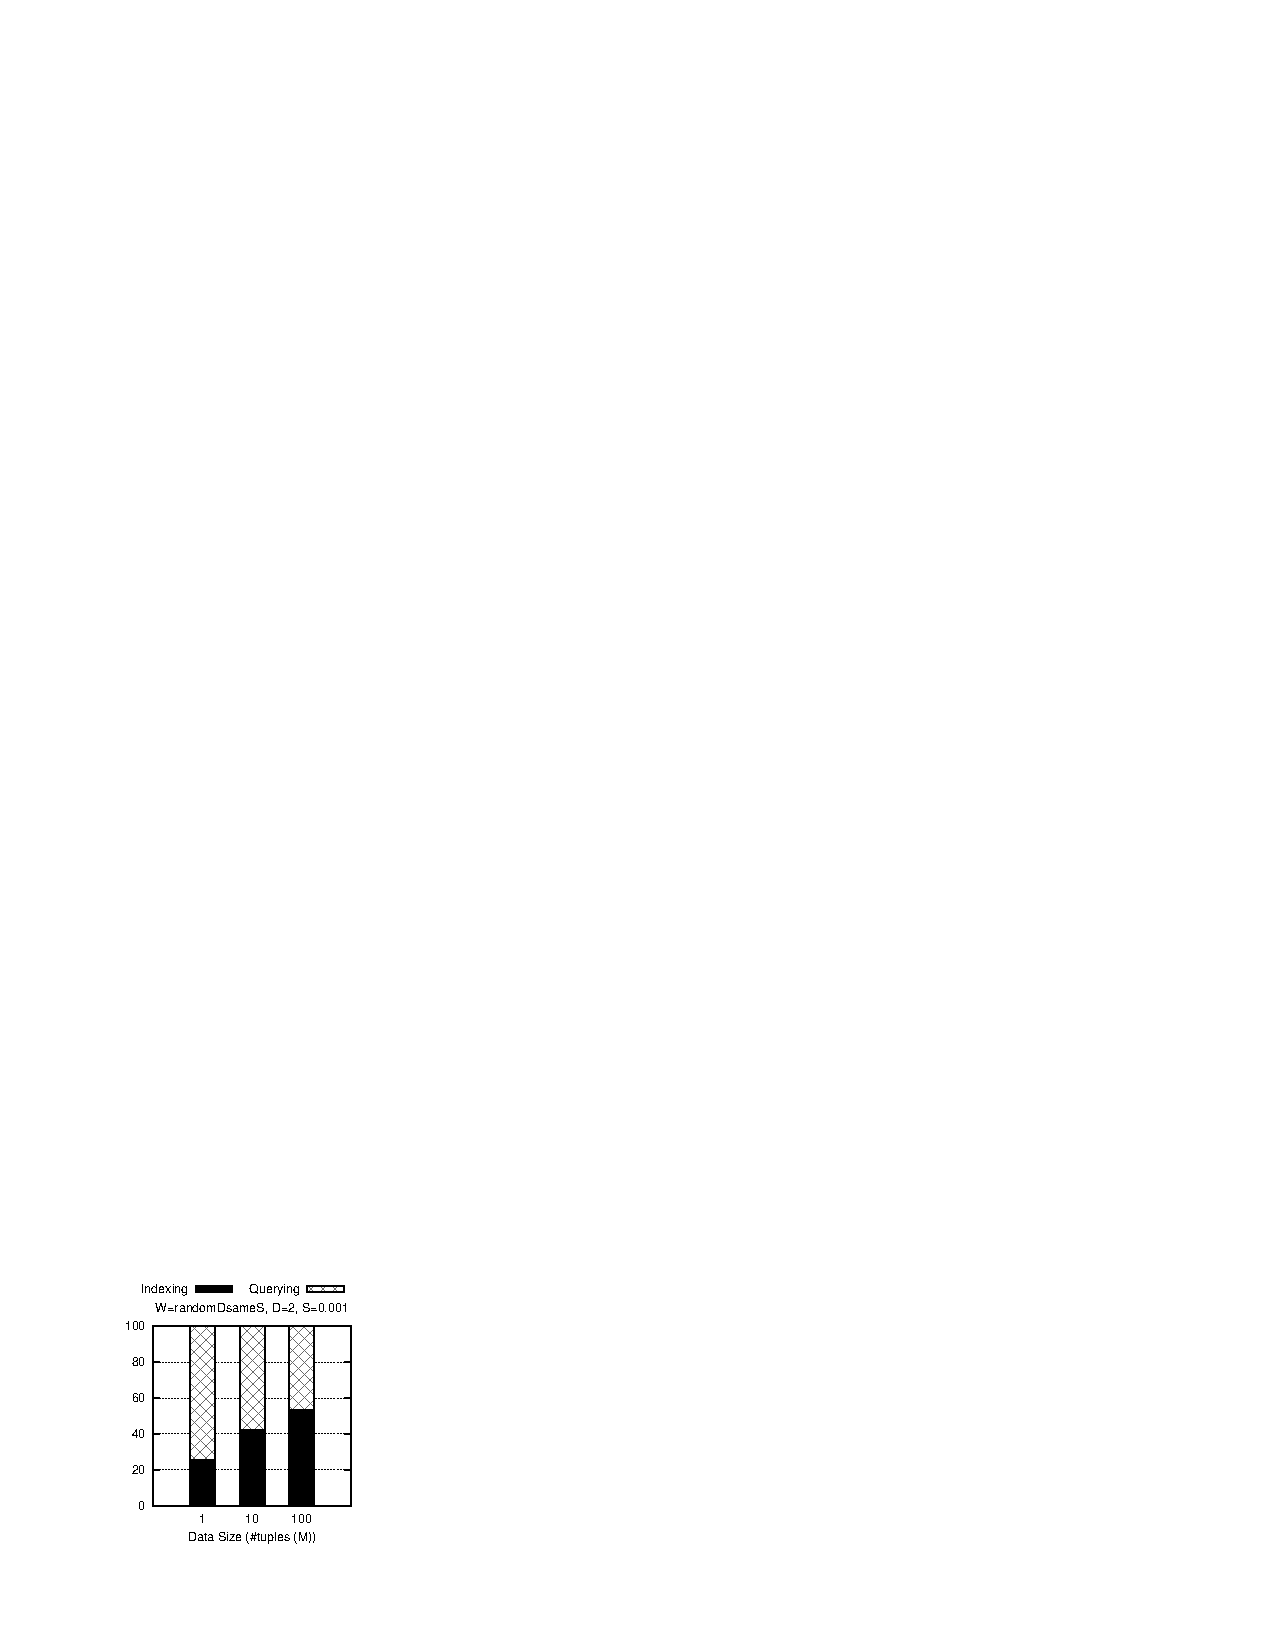
\includegraphics[trim=2cm 2.1cm 15cm 22cm]{Figures/data_to_query_gap/graph_2_randomDsameS_1_10000}
        }%
	\subfigure[]{%
            \label{fig:randomDsameS001}
            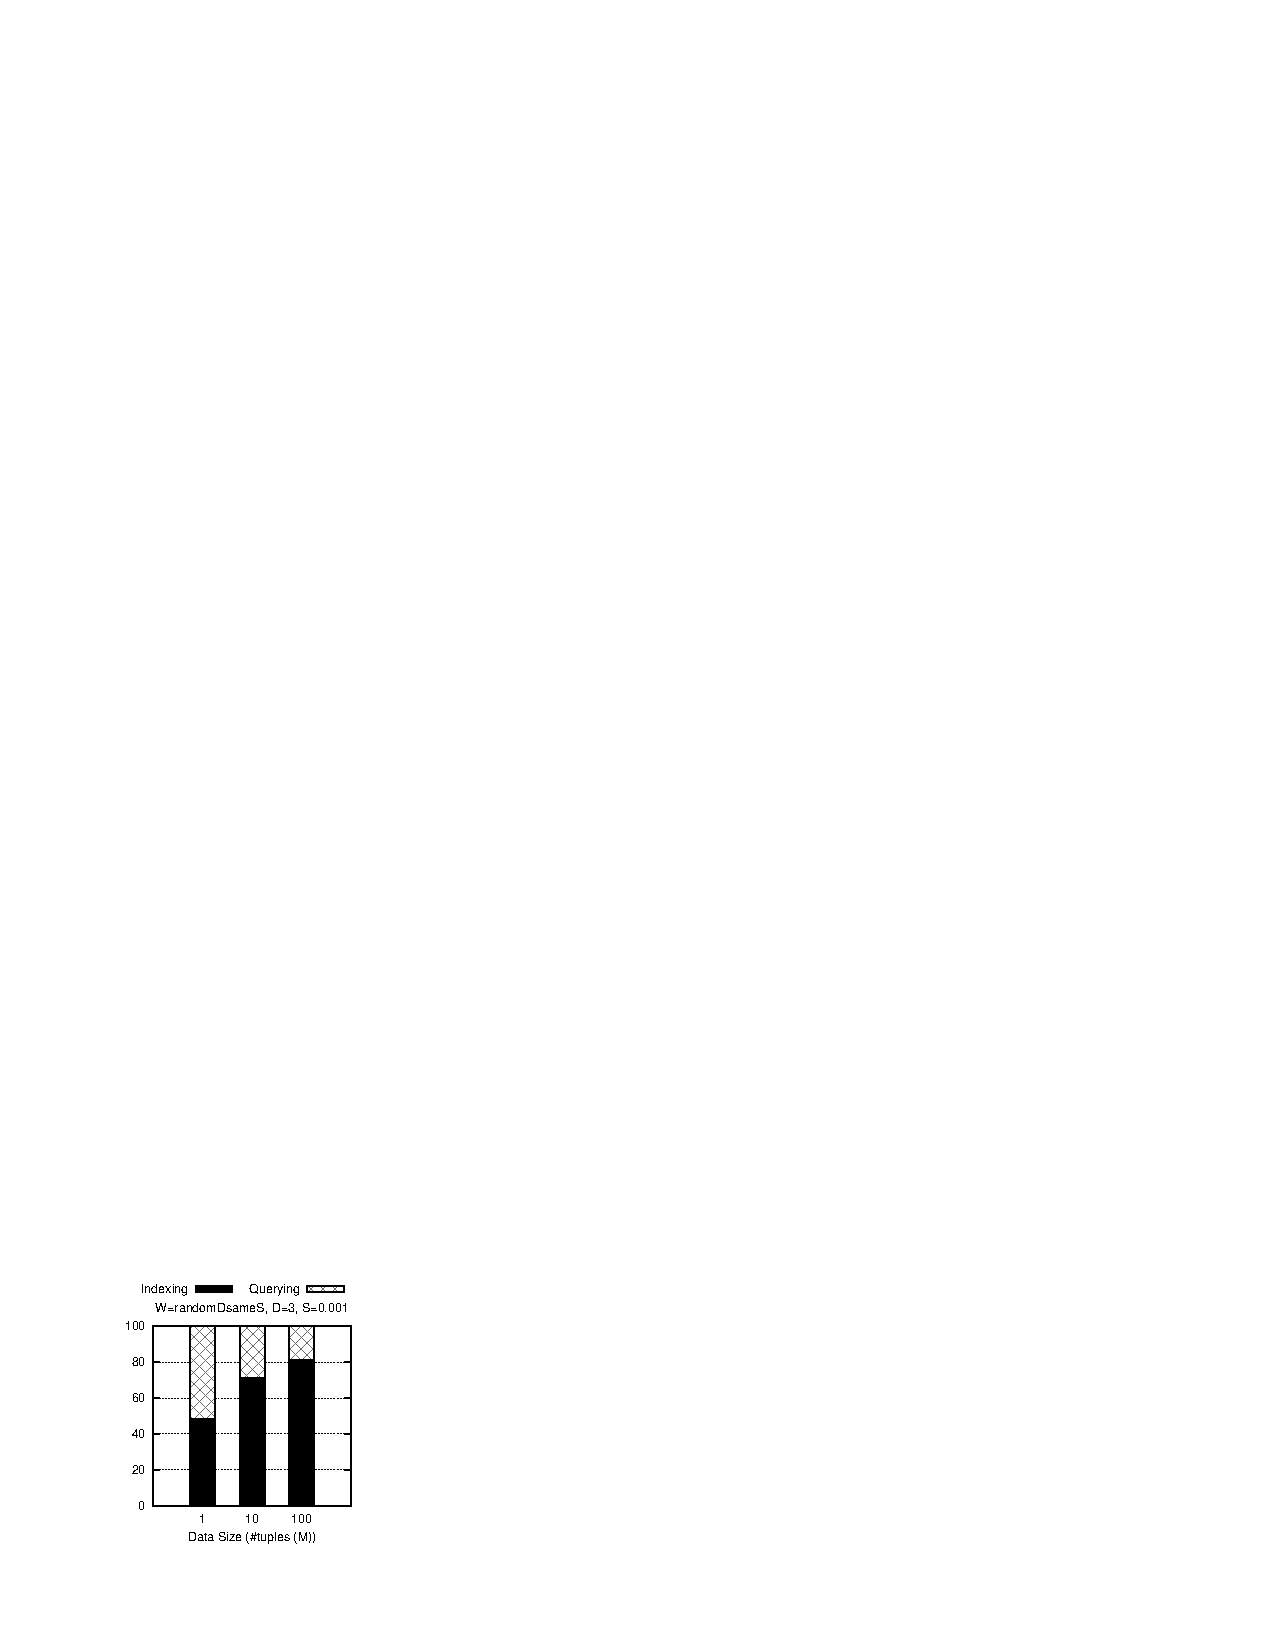
\includegraphics[trim=2.5cm 2.1cm 15cm 22cm]{Figures/data_to_query_gap/graph_3_randomDsameS_1_10000}
        }%
    \caption{The data to query gap: building an index takes more time than answering $10^5$ queries.}
   \label{fig:index_build}
    \end{center}
\end{figure}

Big data exploration cannot be relied on full sequential scans for every query because of the prohibitive scan cost.
Indexing is necessary in order to accelerate query processing in such way that analysts can explore data fast in real time.
Traditional indexing methods build an index that covers all data equally before query processing.
However, we show that the amount of time required to build a full index is a significant bottleneck.
Figure~\ref{fig:index_build} shows the breakdown of the total execution time of 10000 range selection queries over two- and three-dimensional points into the index building cost and the querying cost.
In two dimensions it takes more than 50\% of the time to build a state-of-the-art index (KDTree \cite{DBLP:journals/cacm/Bentley75}) over a data set of 100 million points, while in three dimensions indexing the data takes more than 80\% of the time in a modern server machine.
As the data size grows, the total indexing cost increases dramatically, to a degree where it creates a big and disruptive gap
between the time when the data is available and the time when one can actually have access to the data.   
In fact,  as the data grows, the query processing cost increasingly becomes a smaller fraction of the total cost (indexing + querying).  
We will discuss this experiment and its setup in more detail later on.


\textbf{Data Exploration.}
As data sizes grow even bigger, waiting for long stretches of time before posing the first queries can be a major show-stopper for many applications both in businesses and in sciences.
In addition, firing exploratory queries, i.e., queries which are not known a priori, is becoming quickly a common scenario. 
That is, in many cases, analysts and scientists need to explore the data before they can figure out what the next query is, or even which experiment to perform next; the output of one query inspires the formulation of the next query, and drives the experimental process. 
In such cases, performing tuning and initialization actions up-front suffers from the fact that we do not have enough knowledge about which data parts are of interest, e.g., \cite{Here_are, dbtouch_1, dbtouch_2}. 
Similarly, in many applications, predefined queries are beneficial only if they can track data patterns or events within a given time limit;
 e.g., traffic monitoring applications for advertisement need to quickly determine user positions and interests.

\textbf{Adaptive Multidimensional Indexing.}
We propose an adaptive indexing solution which minimizes the index creation time allowing users to query the data soon after its generation and several times faster compared to state-of-the-art indexing approaches.  
As more queries are posed, the index is continuously refined and subsequent queries enjoy even better execution times. 
Although the concept of adaptive indexing has been studied in the context of column-store databases, there the main goal is to incrementally sort  individual arrays (i.e., columns) for point or range queries.  
In contrast, a multidimensional adaptive index is a tree-based index that is tailored to answer range search queries over general multidimensional records, thus requiring very different techniques, able to simultaneously index multiple arrays.


%\textbf{Contribution.}
%\begin{itemize}
%\item Our hypothesis, e.g., workload is not known a priori, not enough time to build full index, etc.
%\item Our approach, e.g., data structures we need, method, data features, workload features, etc. 
%\end{itemize}
%\textbf{Reader's satisfaction.} Point out what might impress the reader and make clear if what we are doing is reusable by other systems.
\textbf{Contributions.} Our contributions are summarized as follows.
\begin{itemize}
  \setlength{\itemsep}{0pt}
  \setlength{\parskip}{0pt}
  \setlength{\parsep}{0pt}
\item We demonstrate the inability of state-of-the-art indexing to cope with exploratory analysis of very large multi-dimensional data collections. We show that the index creation time is a major bottleneck which becomes worse as data grows.
\item We introduce a novel adaptive clustering technique.  Adaptive clustering minimizes the data to query gap by integrating indexing actions with query processing and being able to immediately process user queries.
The index structure is continuously enriched as more data and queries arrive and only for the hot part of the data.
\item Furthermore,  we  propose adaptive clustering algorithms that automatically expand hot subtrees in the hot branches of the index to minimize querying costs.
\item Through a detailed experimental evaluation with both synthetic and diverse real-world workloads, we show that it is possible to drastically reduce the data to query time, being able to handle thousands of queries by the time that state-of-the-art multidimensional indexing (KDTree \cite{DBLP:journals/cacm/Bentley75}) techniques are still in the index creation phase.
\end{itemize}

\textbf{Paper outline.}
The rest of the paper is organized as follows.
In Section~\ref{sec:related_work} we discuss existing multidimensional index structures.
Section~\ref{sec:adaptive_partitioning} describes multidimensional adaptive indexing providing necessary definitions and discussions over the adaptive index built process and the index structure.
Section~\ref{sec:experiments} describes a thorough experimental analysis with both real and synthetic workloads.
Finally, Section~\ref{sec:conclusions} concludes the paper.

